\documentclass[journal,12pt,twocolumn]{IEEEtran}
%
\usepackage{setspace}
\usepackage{gensymb}
\usepackage{siunitx}
%\doublespacing
\singlespacing

%\usepackage{graphicx}
%\usepackage{amssymb}
%\usepackage{relsize}
\usepackage[cmex10]{amsmath}
%\usepackage{amsthm}
%\interdisplaylinepenalty=2500
%\savesymbol{iint}
%\usepackage{txfonts}
%\restoresymbol{TXF}{iint}
%\usepackage{wasysym}
\usepackage{amsthm}
%\usepackage{iithtlc}
\usepackage{mathrsfs}
\usepackage{txfonts}
\usepackage{stfloats}
\usepackage{bm}
\usepackage{cite}
\usepackage{cases}
\usepackage{subfig}
%\usepackage{xtab}
\usepackage{longtable}
\usepackage{multirow}
%\usepackage{algorithm}
%\usepackage{algpseudocode}
\usepackage{enumitem}
\usepackage{mathtools}
\usepackage{steinmetz}
\usepackage{tikz}
\usepackage{circuitikz}
\usepackage{verbatim}
\usepackage{tfrupee}
\usepackage[breaklinks=true]{hyperref}
%\usepackage{stmaryrd}
\usepackage{tkz-euclide} % loads  TikZ and tkz-base
%\usetkzobj{all}
\usetikzlibrary{calc,math}
\usepackage{listings}
    \usepackage{color}                                            %%
    \usepackage{array}                                            %%
    \usepackage{longtable}                                        %%
    \usepackage{calc}                                             %%
    \usepackage{multirow}                                         %%
    \usepackage{hhline}                                           %%
    \usepackage{ifthen}                                           %%
  %optionally (for landscape tables embedded in another document): %%
    \usepackage{lscape}     
\usepackage{multicol}
\usepackage{chngcntr}
\usepackage{amsmath}

%\usepackage{enumerate}

%\usepackage{wasysym}
%\newcounter{MYtempeqncnt}
\DeclareMathOperator*{\Res}{Res}
%\renewcommand{\baselinestretch}{2}
\renewcommand\thesection{\arabic{section}}
\renewcommand\thesubsection{\thesection.\arabic{subsection}}
\renewcommand\thesubsubsection{\thesubsection.\arabic{subsubsection}}

\renewcommand\thesectiondis{\arabic{section}}
\renewcommand\thesubsectiondis{\thesectiondis.\arabic{subsection}}
\renewcommand\thesubsubsectiondis{\thesubsectiondis.\arabic{subsubsection}}

% correct bad hyphenation here
\hyphenation{op-tical net-works semi-conduc-tor}
\def\inputGnumericTable{}                                 %%

\lstset{
%language=C,
frame=single, 
breaklines=true,
columns=fullflexible
}
%\lstset{
%language=tex,
%frame=single, 
%breaklines=true
%}
\usepackage{graphicx}
\usepackage{pgfplots}

\begin{document}
%


\newtheorem{theorem}{Theorem}[section]
\newtheorem{problem}{Problem}
\newtheorem{proposition}{Proposition}[section]
\newtheorem{lemma}{Lemma}[section]
\newtheorem{corollary}[theorem]{Corollary}
\newtheorem{example}{Example}[section]
\newtheorem{definition}[problem]{Definition}
%\newtheorem{thm}{Theorem}[section] 
%\newtheorem{defn}[thm]{Definition}
%\newtheorem{algorithm}{Algorithm}[section]
%\newtheorem{cor}{Corollary}
\newcommand{\BEQA}{\begin{eqnarray}}
\newcommand{\EEQA}{\end{eqnarray}}
\newcommand{\define}{\stackrel{\triangle}{=}}
\bibliographystyle{IEEEtran}
%\bibliographystyle{ieeetr}
\providecommand{\mbf}{\mathbf}
\providecommand{\pr}[1]{\ensuremath{\Pr\left(#1\right)}}
\providecommand{\qfunc}[1]{\ensuremath{Q\left(#1\right)}}
\providecommand{\sbrak}[1]{\ensuremath{{}\left[#1\right]}}
\providecommand{\lsbrak}[1]{\ensuremath{{}\left[#1\right.}}
\providecommand{\rsbrak}[1]{\ensuremath{{}\left.#1\right]}}
\providecommand{\brak}[1]{\ensuremath{\left(#1\right)}}
\providecommand{\lbrak}[1]{\ensuremath{\left(#1\right.}}
\providecommand{\rbrak}[1]{\ensuremath{\left.#1\right)}}
\providecommand{\cbrak}[1]{\ensuremath{\left\{#1\right\}}}
\providecommand{\lcbrak}[1]{\ensuremath{\left\{#1\right.}}
\providecommand{\rcbrak}[1]{\ensuremath{\left.#1\right\}}}
\theoremstyle{remark}
\newtheorem{rem}{Remark}
\newcommand{\sgn}{\mathop{\mathrm{sgn}}}
\providecommand{\abs}[1]{\left\vert#1\right\vert}
\providecommand{\res}[1]{\Res\displaylimits_{#1}} 
\providecommand{\norm}[1]{\left\lVert#1\right\rVert}
%\providecommand{\norm}[1]{\lVert#1\rVert}
\providecommand{\mtx}[1]{\mathbf{#1}}
\providecommand{\mean}[1]{E\left[ #1 \right]}
\providecommand{\fourier}{\overset{\mathcal{F}}{ \rightleftharpoons}}
%\providecommand{\hilbert}{\overset{\mathcal{H}}{ \rightleftharpoons}}
\providecommand{\system}{\overset{\mathcal{H}}{ \longleftrightarrow}}
	%\newcommand{\solution}[2]{\textbf{Solution:}{#1}}
\newcommand{\solution}{\noindent \textbf{Solution: }}
\newcommand{\cosec}{\,\text{cosec}\,}
\providecommand{\dec}[2]{\ensuremath{\overset{#1}{\underset{#2}{\gtrless}}}}
\newcommand{\myvec}[1]{\ensuremath{\begin{pmatrix}#1\end{pmatrix}}}
\newcommand{\mydet}[1]{\ensuremath{\begin{vmatrix}#1\end{vmatrix}}}
%\numberwithin{equation}{section}
\numberwithin{equation}{subsection}
%\numberwithin{problem}{section}
%\numberwithin{definition}{section}
\makeatletter
\@addtoreset{figure}{problem}
\makeatother
\let\StandardTheFigure\thefigure
\let\vec\mathbf
%\renewcommand{\thefigure}{\theproblem.\arabic{figure}}
\renewcommand{\thefigure}{\theproblem}
%\setlist[enumerate,1]{before=\renewcommand\theequation{\theenumi.\arabic{equation}}
%\counterwithin{equation}{enumi}
%\renewcommand{\theequation}{\arabic{subsection}.\arabic{equation}}
\def\putbox#1#2#3{\makebox[0in][l]{\makebox[#1][l]{}\raisebox{\baselineskip}[0in][0in]{\raisebox{#2}[0in][0in]{#3}}}}
     \def\rightbox#1{\makebox[0in][r]{#1}}
     \def\centbox#1{\makebox[0in]{#1}}
     \def\topbox#1{\raisebox{-\baselineskip}[0in][0in]{#1}}
     \def\midbox#1{\raisebox{-0.5\baselineskip}[0in][0in]{#1}}
\vspace{3cm}
\title{Matrix Theory (EE5609) Challenging Problem 1}
\author{Arkadipta De\\MTech Artificial Intelligence\\AI20MTECH14002}

\maketitle
\newpage
%\tableofcontents
\bigskip
\renewcommand{\thefigure}{\theenumi}
\renewcommand{\thetable}{\theenumi}

\begin{abstract}
This document explains the concept of finding the closest points on two skew lines in 3-Dimensions.
\end{abstract}
The code for the solution of this problem can be found at
%
\begin{lstlisting}
https://github.com/Arko98/EE5609/blob/master/Challenge_1/Codes/Figure.py
\end{lstlisting}
%
\section{Problem}
Find the points on two skew lines that are closest to each other in 3-Dimensions.
\section{Explanation}
Let, skew line, $\vec{L_1}$ is passing through the point $A(a_1,b_1,c_1)$ with direction vector $(D_1(l_1,m_1,n_1)$ and skew line, $\vec{L_2}$ is passing through the point $B(a_2,b_2,c_2)$  with direction vector $(D_2(l_2,m_2,n_2)$. The equations of skew lines are given by,
\begin{align}
\vec{L_1}: \vec{r_1}&=A+k_1(\vec{D_1})\label{eq1}\\
\vec{L_2}: \vec{r_2}&=B+k_2(\vec{D_2})\label{eq2}
\end{align}
Where $r_1=\myvec{x_1\\y_1\\z_1}$ and $r_2=\myvec{x_2\\ y_2\\z_2}$ be two arbitrary points on skew lines $\vec{L_1}$ and $\vec{L_2}$, respectively. \\
Let, the closest points on skew lines $\vec{L_1}$ and $\vec{L_2}$ be $\vec{P}$ and $\vec{Q}$, respectively. Hence $\vec{P}$ and $\vec{Q}$ can be expressed in terms of equation \eqref{eq1} and \eqref{eq2},
\begin{align}
\vec{P}=\myvec{a_1+k_1l_1\\b_1+k_1m_1\\c_1+k_1n_1}\label{eq3}\\
\vec{Q}=\myvec{a_2+k_2l_2\\b_2+k_2m_2\\c_2+k_2n_2}\label{eq4}
\end{align}
So, the position vector from $\vec{P}$ to $\vec{Q}$ i.e $\vec{Q-P}$ is given by, 
\begin{align}
\vec{(Q-P)}=\myvec{a_2+k_2l_2-(a_1+k_1l_1)\\b_2+k_2m_2-(b_1+k_1m_1)\\
c_2+k_2n_2-(c_1+k_1n_1)}\label{eq5}
\end{align}
Since the points $\vec{P}$ and $\vec{Q}$ are closest points, position vector $\vec{PQ}$ will be perpendicular to both the skew lines $\vec{L_1}$ and $\vec{L_2}$ or will be perpendicular to both the direction vectors $\vec{D_1}$ and $\vec{D_2}$.\\ 
Therefore,
\begin{align}
\vec{(Q-P)}\cdot\vec{D_1}&=0\\
\implies(\vec{Q-P})^T\vec{D_1}&=0\label{eq6}
\end{align}
And,
\begin{align}
\vec{(Q-P)}\cdot\vec{D_2}&=0\\
\implies(\vec{Q-P})^T\vec{D_2}&=0\label{eq7}
\end{align}
By solving equations \ref{eq6} and \ref{eq7} we will get $k_1$ and $k_2$. Substituting the obtained values of $k_1$ and $k_2$ in equation \ref{eq3} and \ref{eq4} gives the closest points $\vec{P}$ and $\vec{Q}$.

\section{solution}
Let us illustrate the above approach using an example. Let, the equations of skew lines are given by,
\begin{align}
\vec{L_1}: \vec{r_1}&=\myvec{1\\2\\3}+k_1\myvec{1\\-3\\2}\label{eqL1}\\
\vec{L_2}: \vec{r_2}&=\myvec{4\\5\\6}+k_2\myvec{2\\3\\1}\label{eqL2}
\end{align} 
So, if $\vec{P}$ and $\vec{Q}$ are the points on the skew lines $\vec{L_1}$ and $\vec{L_2}$, then from equation \ref{eq5} the position vector $\vec{Q-P}$ is given by,
\begin{align}
\vec{Q-P}&=\myvec{4+2k_2-(1+k_1)\\5+3k_2-(2-3k_1)\\6+k_2-(3+2k_1)}\\
\implies\vec{Q-P}&=\myvec{-k_1+2k_2+3\\3k_1+3k_2+3\\-2k_1+k_2+3}
\end{align}
Now from equation \ref{eq6} and \ref{eq7}, we get the two equations for $k_1$ and $k_2$ i.e
\begin{align}
\myvec{14&5\\5&14}\myvec{k_1\\k_2} = \myvec{0\\-18}\label{eqS}
\end{align}
Solving the system of equations \ref{eqS}, we get 
\begin{align}
\myvec{k_1\\k_2} = \myvec{\frac{10}{19}\\\frac{28}{19}}
\end{align}
Thus putting the value of $k_1$ in equation \ref{eq3} and putting the value of $k_2$ in equation \ref{eq4} we get $\vec{P}$ and $\vec{Q}$ points as follows,
\begin{align}
\vec{P}&=\myvec{\frac{29}{19}\\\frac{8}{19}\\\frac{77}{19}}=\myvec{1.52\\0.42\\4.05}\\
\vec{Q}&=\myvec{\frac{20}{19}\\\frac{11}{19}\\\frac{86}{19}}=\myvec{1.05\\0.57\\4.52}
\end{align}
Below is the figure corresponding to the solution.
\renewcommand{\thefigure}{\arabic{figure}}
\begin{figure}[h!]
\centering
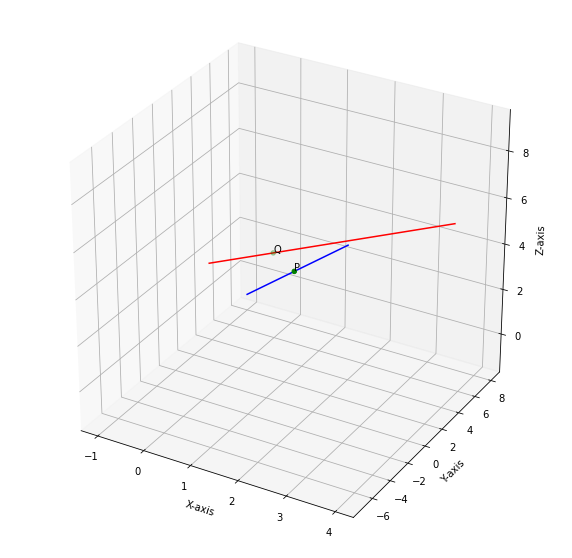
\includegraphics[width=\columnwidth]{Closest_Point.png}
\caption{Closest Points on Skew Lines}
\label{myfig}
\end{figure}\\
\end{document}
